\subsection{Data pre-processing}

As mentioned in the previous section, a public dataset offered by the company \textit{Divvy} has been used \cite{divvy}. This dataset contains the history of all the journeys recorded from 2004 to 2019 in the city of Chicago. This data is offered divided into parts: either by quarters or by months. The final dataset contains $26,328,986$ trips in the entire network with a total of $633$ stations. For each trip, there are $12$ labels associated with them. A sample of the data collected in the dataset can be seen in Appendix \ref{app:original_dataset}.
\newline


For the development of this project, four different modules have been created. Each of these modules will result in a data structure stored in \acrshort{csv} except for the window generator module which will contain information that will be useful for the next module. The main reason why the first two modules result in the creation of a file is to save unnecessary computation time each time a model is to be trained. As training the models requires a multitude of tests with different configurations, it is a process that would have been repeated continuously and whose result would always have been the same. On the other hand, the window generator, a module that will be explained later, being a module that is instantaneous and that also generates different results depending on the model to be developed, does not save the result in any file.
\newline

\begin{figure}[H]
    \centering
    
\includegraphics[width=15cm]{images/solution/modules/modules.png}
    \caption{Project structure divided by modules.}
\end{figure}

During the following sections each of these modules will be explained in detail including diagrams and code.

\subsubsection{\textit{Feature selection} - Unión de \textit{datasets} y filtro de variables}\label{feature-selection}

El \textit{dataset} original \cite{divvy} está divido en años y cada año en múltiples partes. Por lo tanto, la primera tarea de todas ha sido la unión de cada una de estas partes en un único fichero. El formato de archivo ofrecido por \textit{Divvy} es en un CSV como es normal, y por ello se ha usado principalmente la función \verb|read_csv| de pandas que convierte un CSV a un \verb|DataFrame|. Por otro lado, cada parte tenía su propia nomenclatura de columnas por lo que ha sido necesario crear una única nomenclatura para poder trabajar con un único fichero y por ello han sido renombradas algunas columnas. Una vez realizado el renombrado de columnas, el \verb|DataFrame| será anexionado a otro que contendrá todos los datos y que será el que se usará para los siguientes pasos.

\begin{displayquote}
"Un \verb|DataFrame| es una estructura de datos etiquetada en 2 dimensiones con columnas de tipos potencialmente diferentes. Se puede pensar en ello como una hoja de cálculo o una tabla SQL. Generalmente es el objeto más comúnmente usado en la librería de \textit{pandas}." \cite{pandas}
\end{displayquote}

Un ejemplo de \verb|DataFrame| que se ha visto con anterioridad podría ser la tabla \ref{tab:houses}. Para poder inicializar un \verb|DataFrame| se puede realizar desde un diccionario de Python, donde cada clave sea el \verb|string| que identifica a la columna y cada valor sea un vector con la misma cantidad de valores que filas quiere que se tenga. Otra forma de inicializar un \verb|DataFrame| es mediante el uso de funciones como \verb|read_csv()|, \verb|read_h5()| o \verb|read_pickle()|.
\newline

El código usado es algo parecido a lo que se muestra a continuación:

\begin{minted}[fontsize=\footnotesize]{python}
import pandas as pd

# Path to the csv files
csv_filenames = ["trips-2014-Q1", "trips-2014-Q2-Q3", 
                 "trips-2014-Q4", "trips-2015-Q1-Q2",
                 # ...
                 "trips-2019-Q3-Q4"]
csv_paths = [f"/path/to/{file}.csv" for file in csv_filenames]

# This will be the final DataFrame
df = pd.DataFrame()

# For every CSV do
for path in csv_paths:
    
    # CSV to DataFrame
    df_temp = pd.read_csv(path)
    
    # Parse date as datetime which is always first column
    df_temp[cols[0]] = pd.to_datetime(
        df_temp[cols[0]], 
        format='%Y-%m-%d %H:%M:%S',
        infer_datetime_format=True)
    
    # Rename the columns depending on their
    # current names with a external function
    df_temp = rename_columns(df_temp)
    
    # Merge the DataFrames
    df = pd.concat([df, df_temp], join='outer')

# ...
\end{minted}

Una vez obtenido la variable \verb|df| con todos los viajes, se necesita realizar un filtro de las columnas. En este punto, el \verb|DataFrame| contine 12 valores asociados a cada viaje.

\begin{minted}[fontsize=\footnotesize]{python}
df.columns

'''
Index(['trip_id', 'start_time', 'end_time', 'bikeid', 
       'tripduration', 'from_station_id', 
       'from_station_name', 'to_station_id',
       'to_station_name', 'usertype', 'gender',
       'birthyear'],
      dtype='object')
'''
\end{minted}

De este \verb|DataFrame| solo se seleccionan dos:

\begin{itemize}
    \item \textit{start\_time}: Este dato es necesario porque se quiere predecir el uso de bicicletas a partir de una información temporal. Este valor, dado en segundos usando el formato "Tiempo Unix" \cite{unix_time}, nos permite identificar en qué fecha y hora se inició el viaje. Gracias a ello, se pueden identificar distintos patrones, ya que estos varían durante la época del año. No existen los mismos patrones durante el invierno que durante el verano o incluso, no es lo mismo las 2 de la madrugada que las 2 de la tarde.
    \item \textit{from\_station\_id}: Los modelos que se van a construir predecirán el número de viajes que se inician en cada estación de Chicago de forma independiente. Este valor por tanto, será usado para calcular el número de viajes iniciados en un intervalo en cada estación.
\end{itemize}

El resto de atributos también son útiles para otro tipos de problemas como por ejemplo predecir el destino más probable en función de la estación donde se inicia el viaje, u obtener que conexiones son las más transitadas. Sin embargo, está fuera de los objetivos que se han planteado para este trabajo por lo que solo se usarán las columnas previamente mencionadas.
\newline
 
El dataset resultante por tanto, es el mismo dataset original pero con solo las columnas \textit{start\_time} y \textit{from\_station\_id}. En el código esto es fácil de implementar añadiendo solo la siguientes línea:
\begin{minted}[fontsize=\footnotesize]{python}
# ...
    
# Filter the columns that we need
cols = ["start_time", "from_station_id"]
df = df[cols]

# Save the DataFrame in a CSV
df.to_csv("trips.csv", index=False)
\end{minted}

Se podrían haber usado más columnas que ayudasen a la predicción, sin embargo, por falta de tiempo y porque los resultados obtenidos eran de por sí bastante buenos, no se ha visto la necesidad de añadirlos.
\newline

Gráficamente este módulo realiza lo siguiente:
\begin{figure}[H]
    \centering
    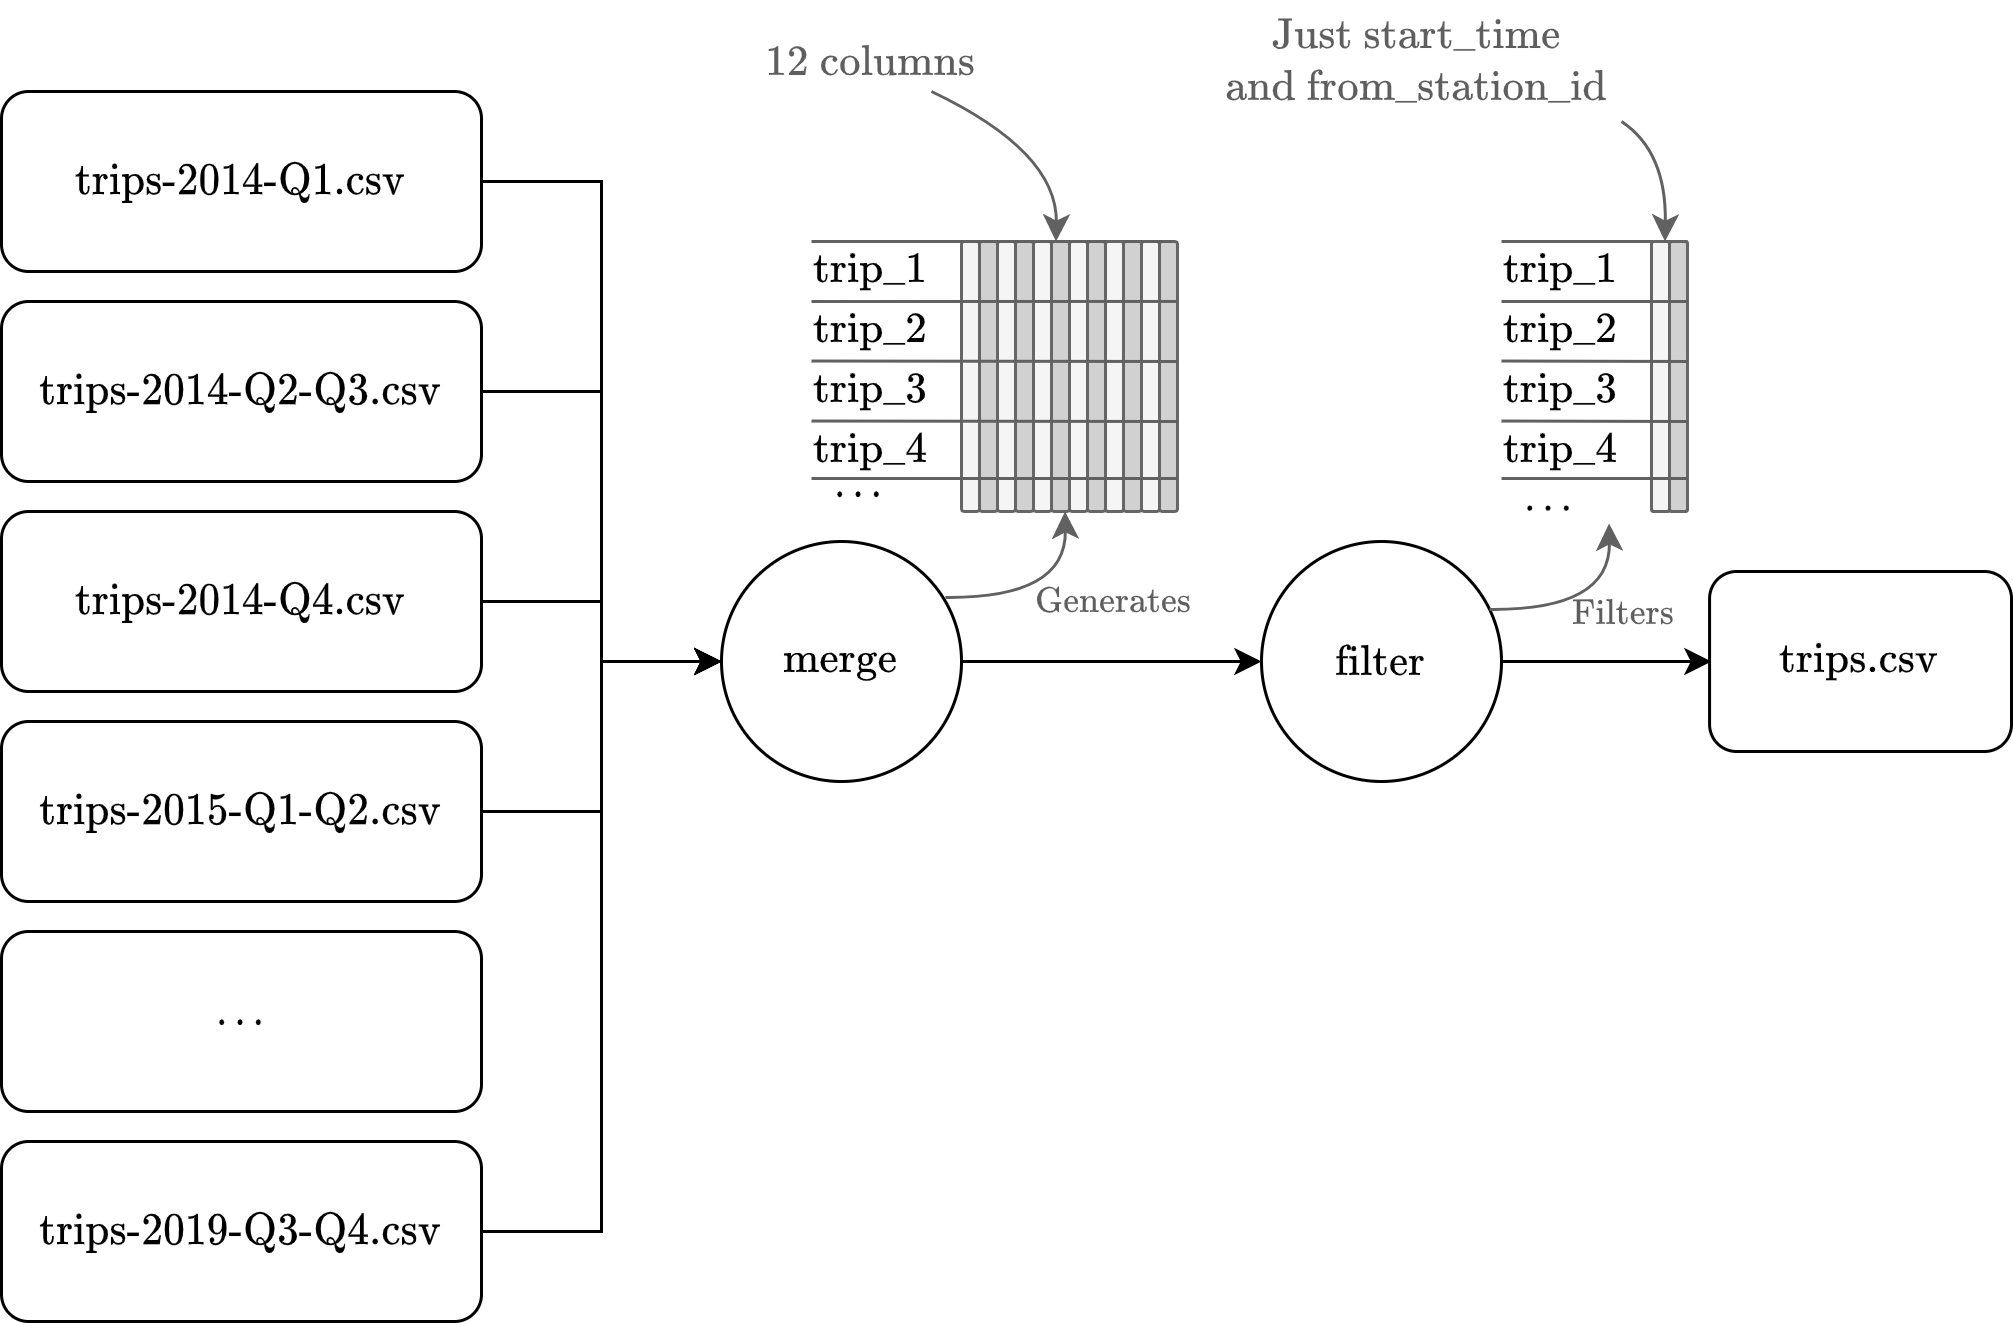
\includegraphics[width=12cm]{images/solution/modules/feature-selection.png}
    \caption{Estructura del módulo \textit{feature-selection}.}
\end{figure}
\subsubsection{Definición de entradas y salidas de las redes neuronales}\label{inputs-outputs}

Antes de continuar explicando los pasos llevados a cabo hay que diseñar que \textit{dataset} se necesita para entrenar a las redes neuronales. Uno de los principales requisitos en el diseño de redes neuronales es la correcta especificación del vector de entrada y salida de la red neuronal. La cantidad de variables y el tipo de variables que se usarán en la red es una de las principales claves para que el modelo funcione de forma satisfactoria. En este apartado se explicará tanto la estructura del vector de entrada como la estructura del vector de salida acompañado de ejemplos gráficos.
\newline

Los modelos con los que trabajaremos tendrán como entrada valores que representan la fecha y la hora representados con los siguientes atributos: \textit{hour} (h), \textit{day\_of\_week}(d) y \textit{month}(m). Es decir, los viajes se agruparan por intervalos, creando de este modo una nueva columna que se denominará \textit{quantity\_$j$} (q), siendo $j$, el índice de la estación. En total hay $633$ estaciones en la ciudad de Chicago. Por lo que para cada intervalo, la red neuronal contará con $636$ valores de entrada. Se pueden ver ejemplos gráficos en la Figura \ref{fig:models-design-1} y \ref{fig:models-design-2}.
\newline

Si se quiere usar más intervalos para que la red entrene, el vector resultante tendrá un número de elementos múltiplo de $636$. Por ejemplo, si se quieren usar 5 intervalos como vector de entrada, entonces la red tendrá una primera capa con $636 \times 5 = 3180$ unidades o neuronas. Por otro lado, se podrían usar más variables conteniendo información importante como puede ser el calendario laboral o variables relacionadas con la meteorología, las cuales influyen en los patrones de comportamiento de la red de bicicletas.
\newline

Por ejemplo, un lunes no laboral, la cantidad de bicicletas alquiladas en un parque será mayor que cualquier otro lunes de otra semana. U otro ejemplo, si un día las condiciones meteorológicas nos son favorables para el uso de bicicleta, la cantidad de bicicletas alquiladas se reducirán considerablemente. Este tipo de variables son algún ejemplo que se podría añadir al \textit{dataset} y así poder mejorar la precisión del modelo pero por falta de tiempo y por simplicidad no se han añadido. Además, los resultados obtenidos de por sí se han considerado bastante buenos y por lo tanto, no se ha visto la necesidad de invertir tiempo en este apartado aunque sería un buen estudio como mejoraría estos modelos con dichos cambios.
\newline

Por otra parte, la salida de la red será un vector que contenga la predicción para todas las estaciones de la red. Es decir, se calculará un vector donde cada valor será la predicción de alguna de las estaciones de la red en un intervalo en concreto. La longitud del vector por lo tanto vendrá dado por el número de estaciones con las que se trabaje, que en total son $633$ multiplicado por la cantidad de intervalos que se quieren predecir, es decir, el vector resultante tendrá $633 \times \text{n\_stations}$ valores. 
\newline

En los modelos autoregresivos, a pesar de ser modelos capaces de predecir múltiples intervalos si fuese neceario, la salida de estos modelos siempre serán de un intervalo. Esto es debido a que es necesario calcular todos los intervalos de forma independiente pues el modelo autoregresivo usa su propia predicción como vector de entrada. Se puede ver más información sobre esto en la Sección \ref{window_ar} y \ref{model_ar}.
\newline

A continuación, se pueden ver gráficamente varios ejemplos de distintas configuraciones de red usando diferentes combinaciones para la cantidad de intervalos de entrada y salida:


\begin{figure}[H]
    \centering
    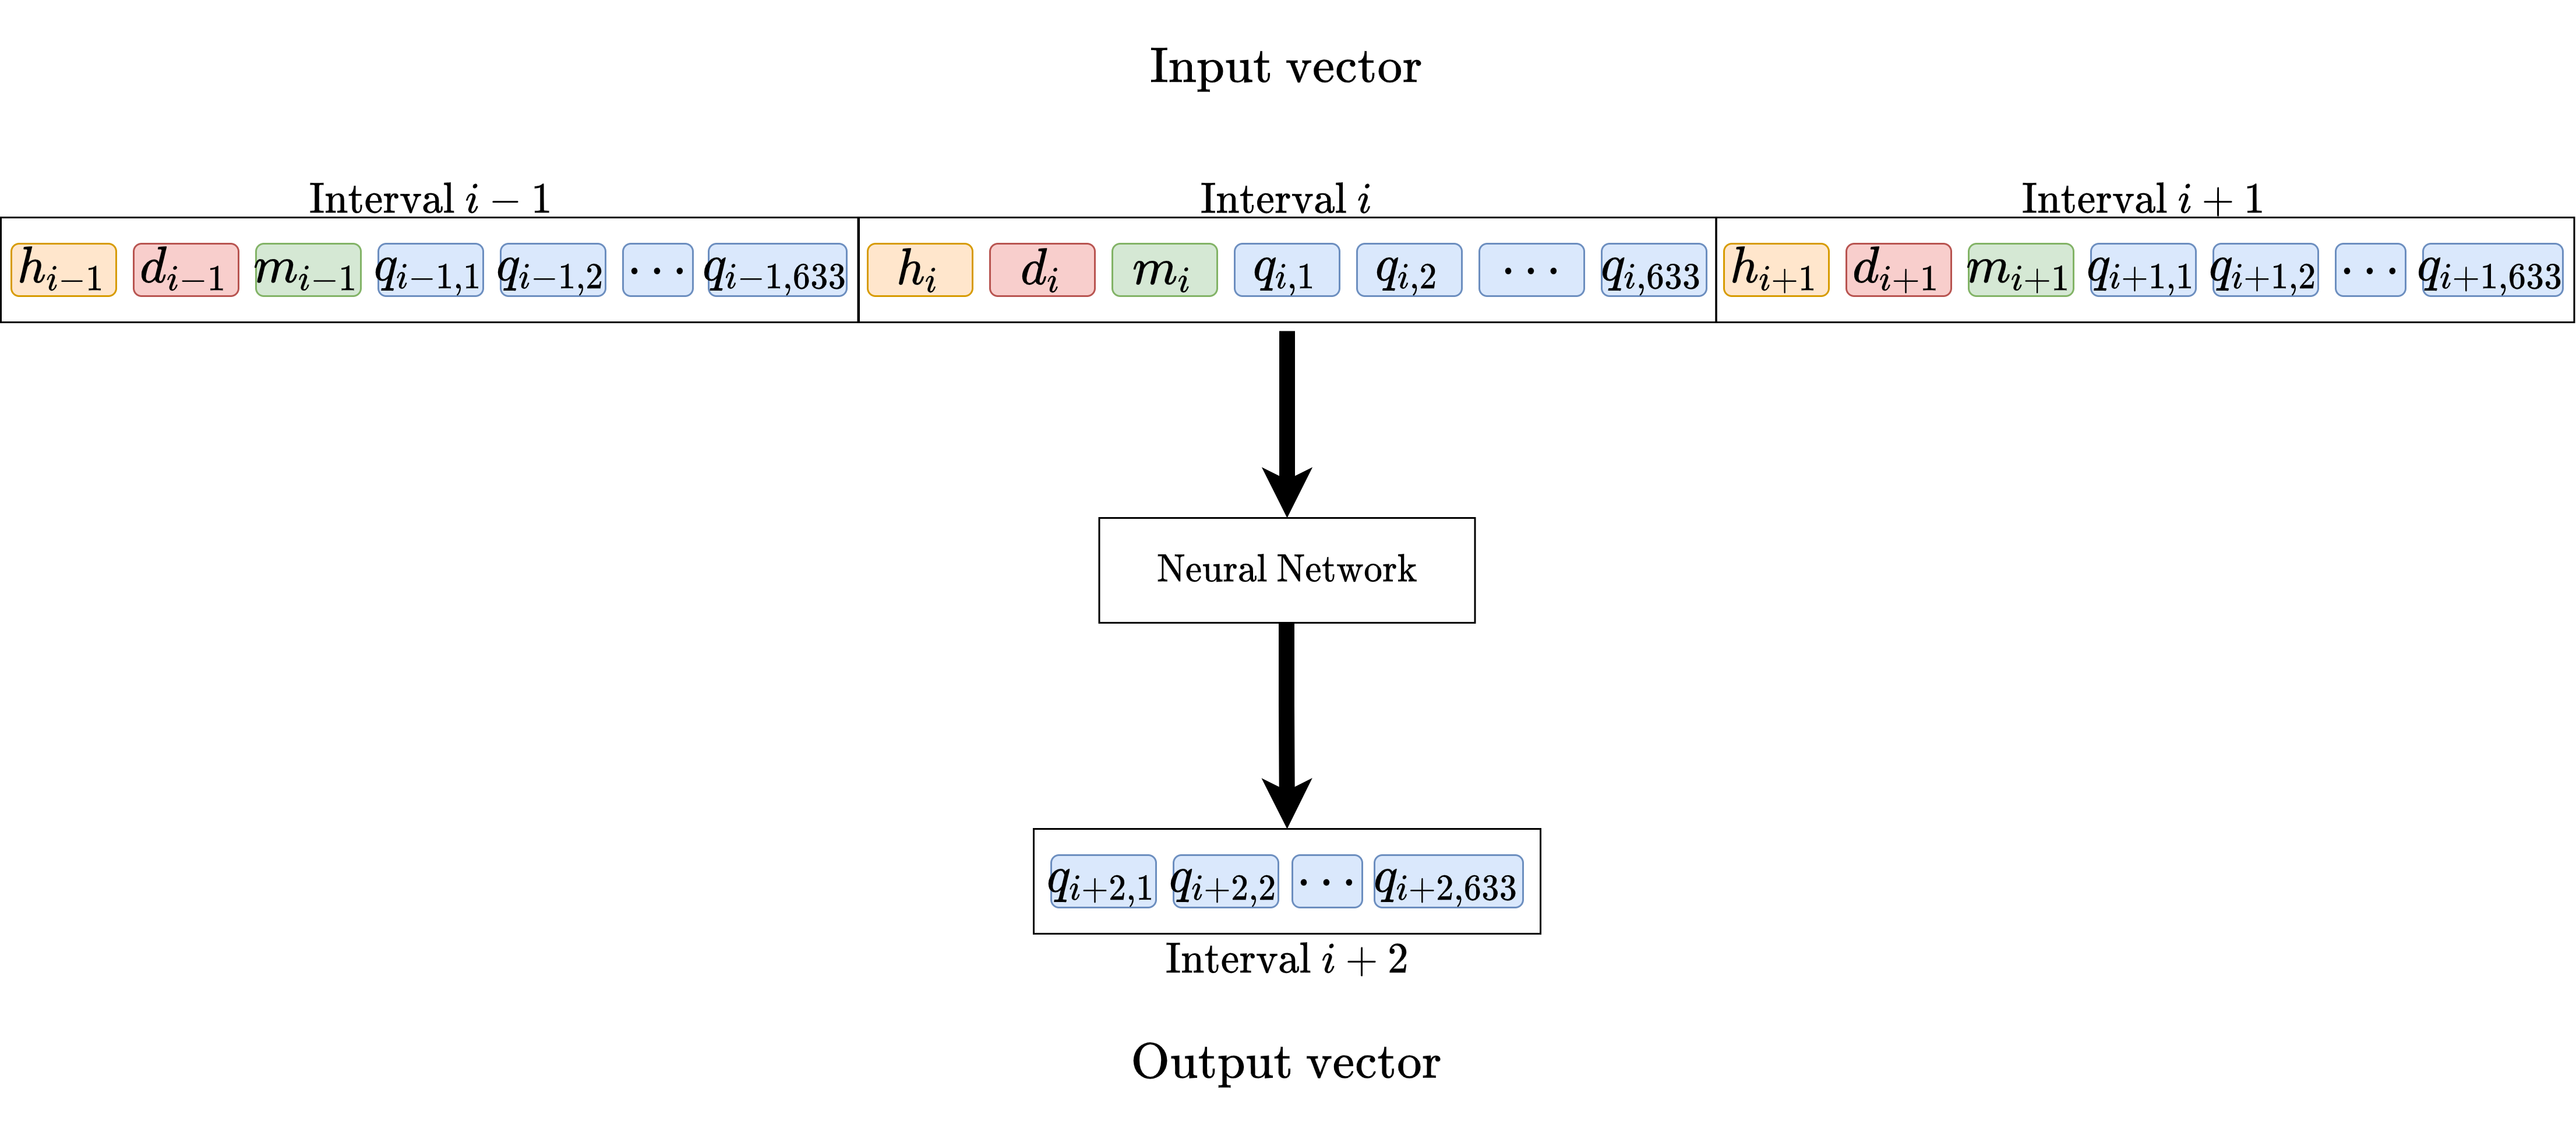
\includegraphics[width=14cm]{images/solution/preprocessing/models-design-1.png}
    \caption{Ejemplo de red neuronal que usa 3 intervalos de entrada y predice 1 intervalo}
    \label{fig:models-design-1}
\end{figure}

\begin{figure}[H]
    \centering
    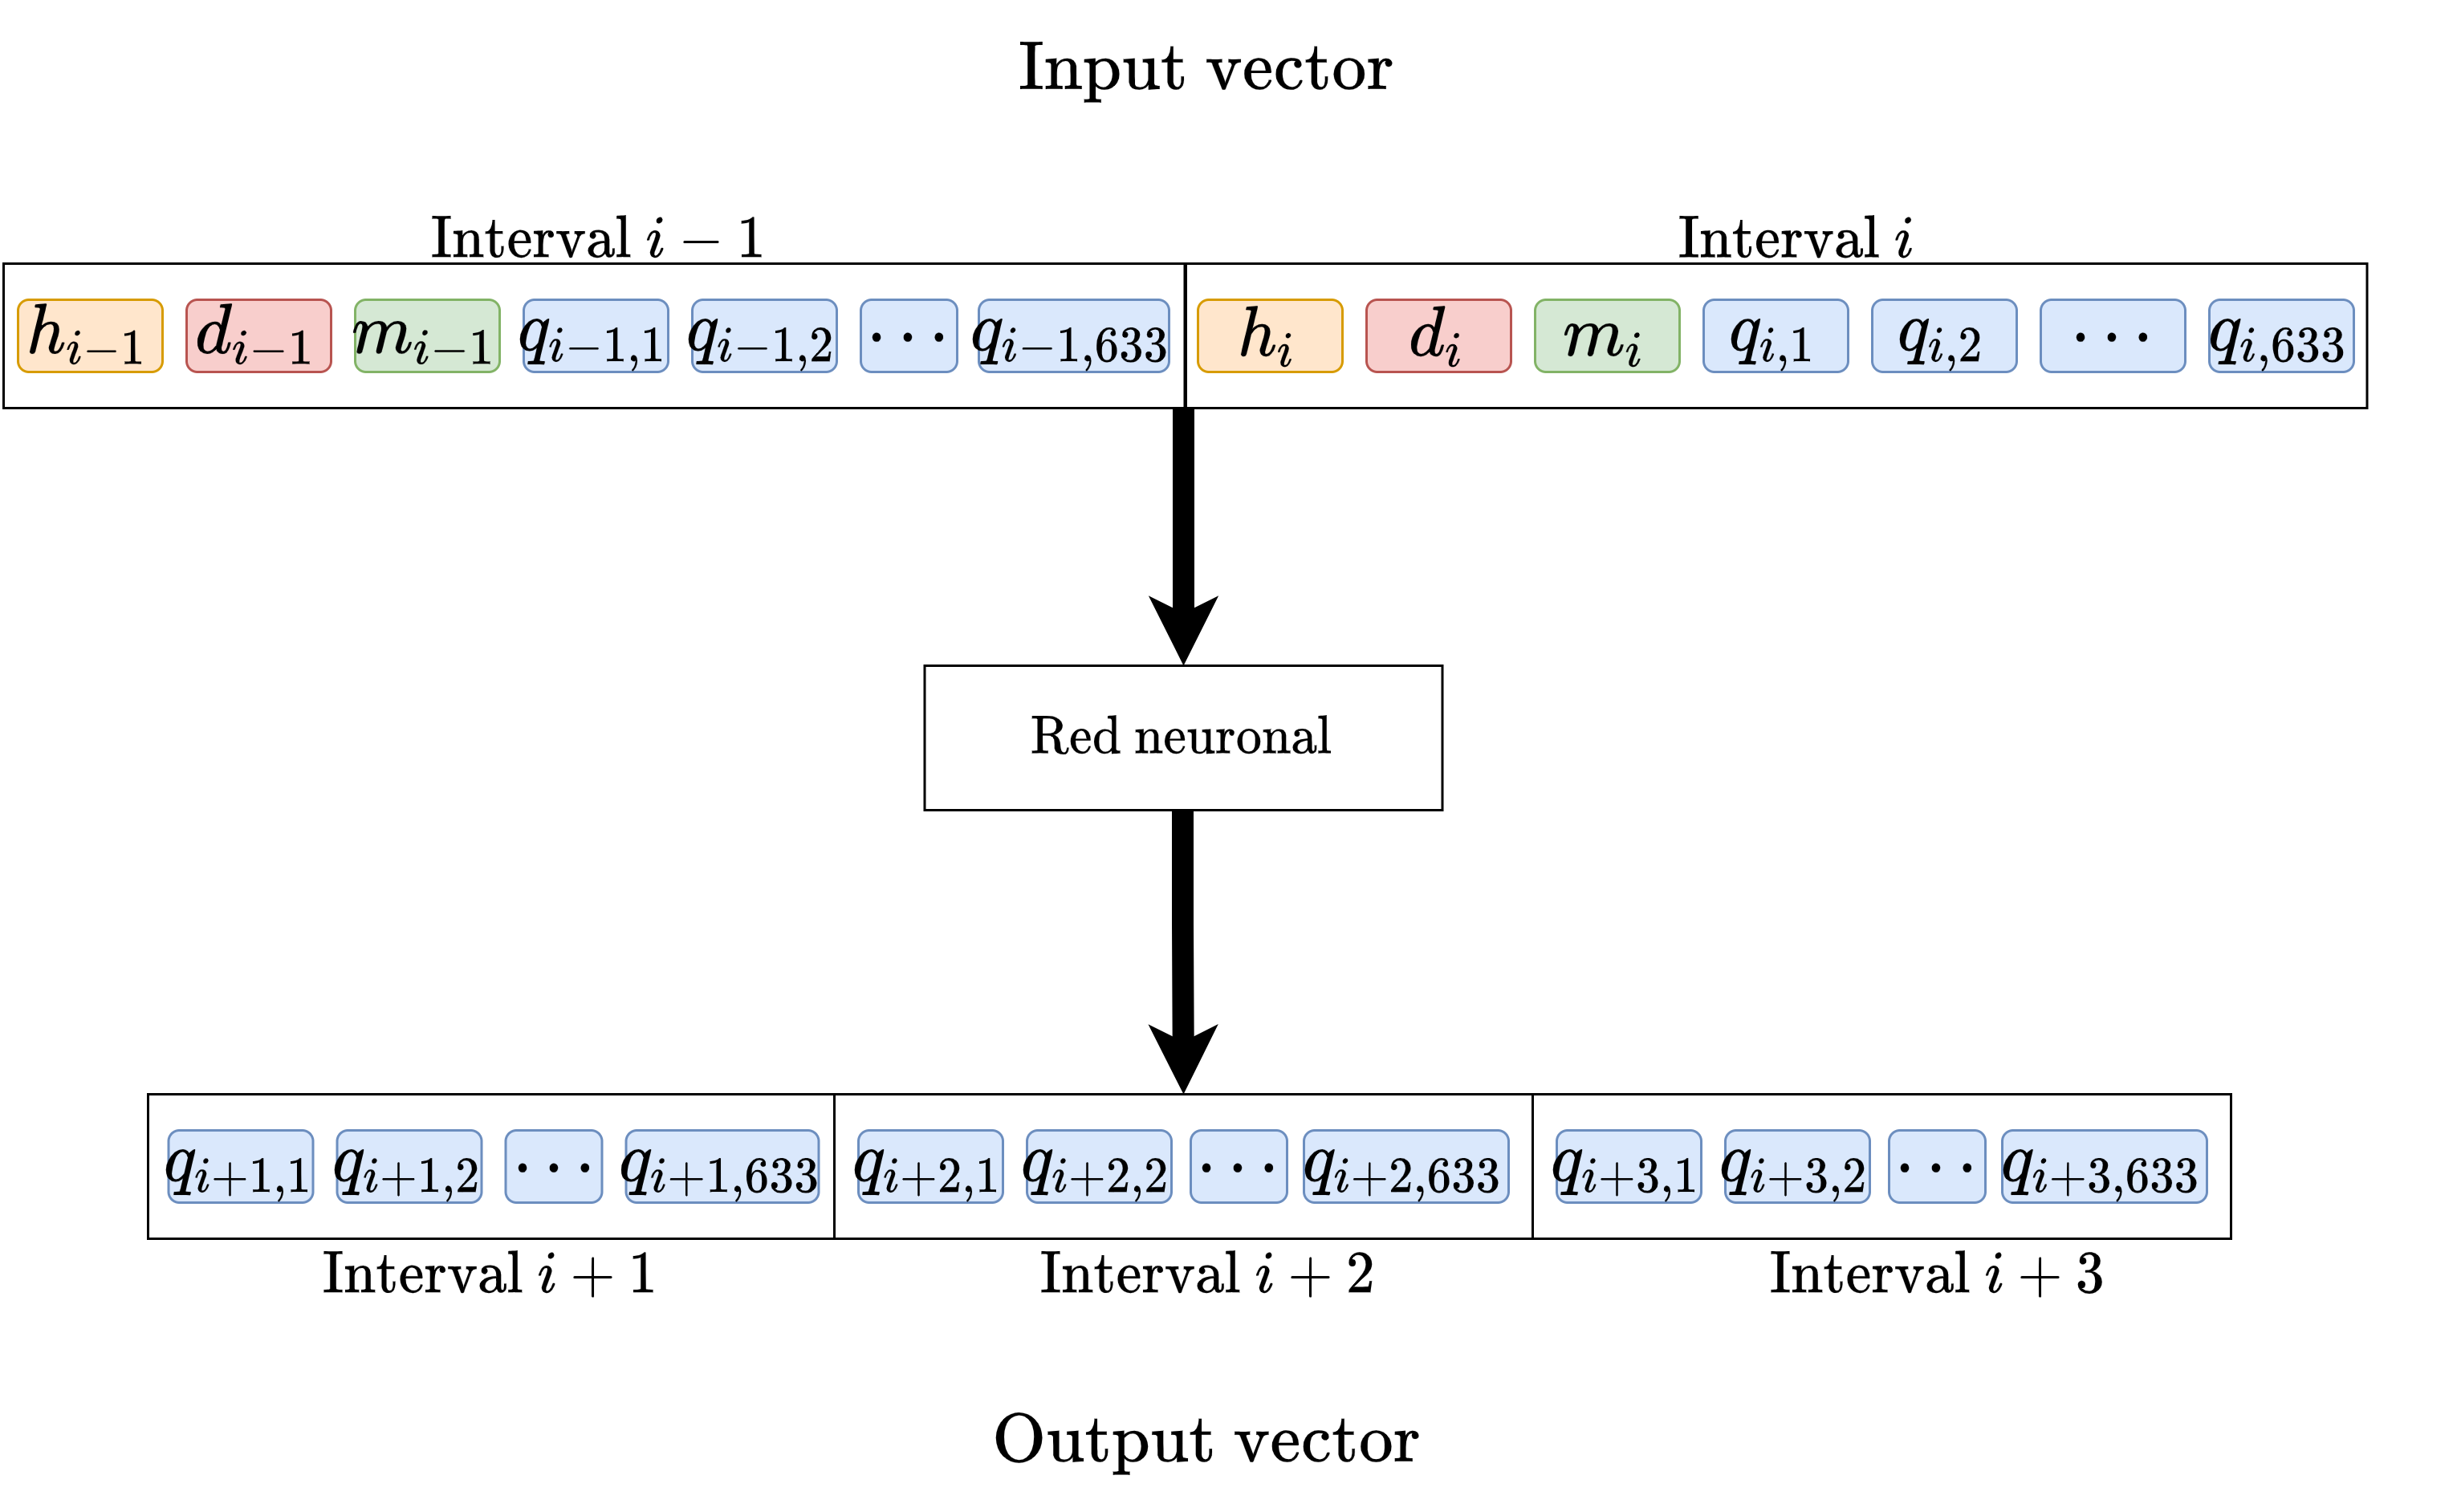
\includegraphics[width=14cm]{images/solution/preprocessing/models-design-2.png}
    \caption{Ejemplo de red neuronal que usa 2 intervalos de entrada y predice 3 intervalos}
        \label{fig:models-design-2}
\end{figure}



Esta estructura, nos permite trabajar con un número variable de estaciones siendo los modelos fácilmente exportables a otras ciudades y otras redes donde la cantidad de estaciones sea distinta. O incluso, si se quisiese trabajar con una única estación se podría realizar sin ningún problema, puesto que cada estación es representada con su propia columna. El código desarrollado para que los modelos funcionen es fácilmente reutilizable para un conjunto de estaciones más pequeñas u otras ciudades o incluso otros problemas de la misma índole, solo haría falta modificar el módulo de \textit{feature-selection} y preprocesamiento.

\subsubsection{Modificando el \textit{dataset} para la red neuronal}\label{dataset-creation}

El \textit{dataset} que se tiene en este punto es un \textit{dataset} que tiene tantas filas como viajes haya habido entre el 2014 y 2019. Por cada fila, se tienen dos atributos: \textit{from\_station\_id} y \textit{start\_time}. 
\newline

En este módulo se quiere modificar dicho \textit{dataset} para obtener un \textit{dataset} que contenga los vectores que puedan ser usados como vectores de entrada en la red. Es decir, se quiere crear un \textit{dataset} que contenga en cada fila los intervalos y en cada columna los datos de dicho intervalo: \textit{hour}, \textit{day\_of\_week}, \textit{month} y \textit{quantity\_$j$}. Al finalizar todos los pasos de este módulo, los datos se guardarán en un archivo llamado \small{\verb|intervals.csv|} y se puede ver una muestra de estos datos en el Apéndice \ref{app:intervals_dataset}.
\newline

Primeramente, el código de este módulo, carga los datos del anterior módulo del archivo CSV \small{\verb|trips.csv|}:
\begin{minted}[fontsize=\footnotesize]{python}
import pandas as pd

# Read CSV as DataFrame an use datetime as index
df = pd.read_csv("/path/to/trips.csv", index="start_time")
\end{minted}

Para poder obtener este dataset, se han tenido que programar una serie de pasos:
\begin{enumerate}
    \item \underline{Agrupar los viajes por intervalos}: Este paso tiene como objetivo agrupar la cantidad de viajes que se inician en cada una de las estaciones en intervalos. Se han estudiado diferentes tamaños de intervalos, como por ejemplo, intervalos de 15 ó 30 minutos, pero finalmente, se ha elegido 1 hora porque se reduce de forma considerable la cantidad de datos y sigue siendo un intervalo válido y no muy amplio.
    \newline
    
    Para este paso lo que se ha realizado ha sido agrupar los distintos viajes en intervalos en función de la columna \textit{from\_station\_id} y \textit{start\_time}. Por ejemplo, teniendo el siguiente \textit{dataset} quese puede ver en la Tabla \ref{tab:starttime_withsid} que contiene ejemplos de viajes, se quiere obtener otro que agrupe por tiempo y por estación como se puede ver en el Tabla \ref{tab:intervals_example}. Para ello primero se agrupara por estación y por intervalo y en el siguiente paso se pivotarán para convertir filas a columnas.
    \newline
    
    Como ejemplo, supongamos que en la variable \small{\verb|df|} se tiene el siguiente \small{\verb|DataFrame|}:

    \begin{table}[H]
    \footnotesize
    \centering
    \begin{tabular}{c|rr}
        \toprule
          \textit{start\_time} & \textit{from\_station\_id}  \\
        \midrule
        
        10:10 - 12/2/2018 & 48\\
        10:28 - 12/2/2018 & 15\\
        10:56 - 12/2/2018 & 15\\
        11:03 - 15/2/2018 & 15\\
        11:12 - 15/2/2018 & 48\\
        11:15 - 15/2/2018 & 15\\
        11:18 - 15/2/2018 & 15\\
        11:31 - 15/2/2018 & 15\\
        11:44 - 15/2/2018 & 48\\
        11:49 - 15/2/2018 & 15\\
        22:00 - 16/2/2018 & 15\\
        22:15 - 16/2/2018 & 48\\
        22:37 - 16/2/2018 & 193\\
        22:56 - 16/2/2018 & 48\\
        \bottomrule
        
    \end{tabular}
    \cprotect\caption{Ejemplo de \textit{dataset} original de \textit{Divvy} que está en \small{\verb|trips.csv|}}
    \label{tab:starttime_withsid}
    \end{table}
    
    Se deben de agrupar los viajes por estación, usando \small{\verb|group_by()|},  \small{\verb|resample()|} y \small{\verb|size()|}. Se puede conseguir esta agrupación usando las siguientes líneas de código:
    
    \begin{minted}[fontsize=\footnotesize]{python}
INTERVAL = "1H"  # It could be also 15Min

df = df.groupby('from_station_id') \
       .resample(INTERVAL, on='start_time') \
       .size() \    # Resampling using the sum rule
       .to_frame()  # Converts it to DataFrame
    \end{minted}
    
    El resultado de este proceso usando el ejemplo de tabla \ref{tab:starttime_withsid} se puede ver en la siguiente tabla:
    
    \begin{table}[H]
    \footnotesize
    \centering
    \begin{tabular}{c|rr}
        \toprule
          \textit{start\_time} & \textit{from\_station\_id} & \textit{quantity}  \\
        \midrule
        
        10:00 - 12/2/2018 & 15 & 2\\
        10:00 - 12/2/2018 & 48 & 1\\
        10:00 - 12/2/2018 & 193 & 0\\
        11:00 - 15/2/2018 & 15 & 5\\
        11:00 - 15/2/2018 & 48 & 2\\
        11:00 - 15/2/2018 & 193 & 0\\
        22:00 - 16/2/2018 & 15 & 1\\
        22:00 - 16/2/2018 & 48 & 2\\
        22:00 - 16/2/2018 & 193 & 1\\
        \bottomrule
    \end{tabular}
    \cprotect\caption{Ejemplo del \textit{dataset} agrupados por estaciones y por intervalos.}
    \label{tab:justintervals}
    \end{table}
    
    

    \item \underline{Pivotar por intervalos}: Este paso tiene como objetivo agrupar todos los intervalos en uno solo, aumentando por tanto la cantidad de columnas reduciendo la cantidad de filas. Es decir, se quiere tener que por cada fila represente un intervalo y por cada columna una estación. Usando el mismo ejemplo del paso anterior, el \small{\verb|DataFrame|} final quedaría de la siguiente manera:
    \begin{table}[H]
    \footnotesize
    \centering
    \begin{tabular}{c|rrr}
        \toprule
        \textit{start\_time} & \textit{quantity\_15} & \textit{quantity\_48} & \textit{quantity\_193}  \\
        \midrule
        10:00 - 12/2/2018 & 2 & 1 & 0 \\
        11:00 - 15/2/2018 & 5 & 2 & 0 \\
        22:00 - 16/2/2018 & 1 & 2 & 1 \\
        
        \bottomrule
    \end{tabular}
    \cprotect\caption{Ejemplo de \textit{dataset} que contiene los intervalos.}
    \label{tab:intervals_example}
    \end{table}
    
    Principalemente, el código usado para este paso hace uso de la función de \textit{pandas} denominada \small{\verb|pivot()|}:
    \begin{minted}[fontsize=\footnotesize]{python}
# Prepare the new columns names for each station
df["quantity_index"] = "quantity_" + \
                        df["from_station_id"].astype("str")

# We don't need from_station_id anymore
df = df.drop(columns=["from_station_id"])

# Make the pivot around quantity_index column and
# set the value of the column the same value as
# quantity from before saving quantity from
df = df.pivot(columns='quantity_index', values='quantity')

# If station any interval didn't have any trips for
# a station, then fill it with 0
return df.fillna(0)
    \end{minted}
    
    \item \underline{Obtener la variables de tiempo}: La columna \textit{start\_time} es una lista con \textit{timestamps} y por lo tanto tiene información más de la necesaria (año, mes, día, hora, minuto, segundo...). La única información temporal que se necesita son un subconjunto de dichos valores. En concreto de los valores que se han creído ser útiles son: la hora, el día de la semana (no es lo mismo un lunes que un sábado) y el mes (no es lo mismo un mes de invierno que de verano). Estos son los valores más simples que se han usado pero eso no quita que se puedan usar otros datos que aportan más información como por ejemplo: día del mes, año o el minuto. 
    \newline
    
    Usando las variables de esta forma y no pasando el \textit{timestamp} directamente a la red, el modelo puede aprender patrones en función de variables más simples como la hora, el día de la semana o el mes, y no con un número de 64 bits que apenas aporta información alguna puesto que la red lo tomaría como valores ascendentes sin ningún tipo de criterio.
    
    Para crear las nuevas columnas con los atributos que se han explicado anteriormente se han usado las siguientes líneas de código:
    \begin{minted}[fontsize=\footnotesize]{python}
# Index and start_time column is the same

df['hour'] = df.index.hour              # Number between 0-23
df['day_of_week'] = df.index.dayofweek  # Number between 0-6
df['month'] = df.index.month            # Number between 1-12
    \end{minted}
    
    Al final de este paso existirán por tanto las siguientes columnas para cada uno de los intervalos: \textit{start\_time}, \textit{hour}, \textit{day\_of\_week}, \textit{month} y una columna por cada estación. La columna \textit{start\_time} no se borra pues es la columna usada como índice y ayuda a la hora de entender la información con la que se trabaja. Pero no será usada por la red neuronal.
    \newline
    
    Usando el mismo ejemplo que los pasos anteriores, la tabla quedaría de la siguiente manera:
    \begin{table}[H]
    \footnotesize
    \centering
    \begin{tabular}{c|rrr|rrr}
        \toprule
        \textit{start\_time} & \textit{quantity\_15} & \textit{quantity\_48} & \textit{quantity\_193} & \textit{hour} & \textit{day\_of\_week} & \textit{month} \\
        \midrule
        10:00 - 12/2/2018 & 2 & 1 & 0 & 10 & 0 & 2 \\
        11:00 - 15/2/2018 & 5 & 2 & 0 & 11 & 3 & 2 \\
        22:00 - 16/2/2018 & 1 & 2 & 1 & 22 & 4 & 2 \\
        
        \bottomrule
    \end{tabular}
    \cprotect\caption{Ejemplo de \textit{dataset} final que será usada por la red neuronal.}
    \label{tab:intervals_example}
    \end{table}
    
    
    En este punto también se estudió la posibilidad de guardar la información de las variables temporales en forma de señal con valores entre los rangos $[-1, 1]$ usando seno y coseno \cite{reddit_time}. Esto permite que el modelo tenga acceso a la información temporal con valores continuos y no discretos como se puede ver en la figura \ref{fig:hour-stepvssignal} a continuación. Los resultados que se obtuvieron con ambas técnicas fueron similares, por lo que por simplicidad se dejo con valores discretos.
    
   \begin{figure}[H]
  \centering
  \subfloat[Hora con valores continuos de $-1$ a $1$]{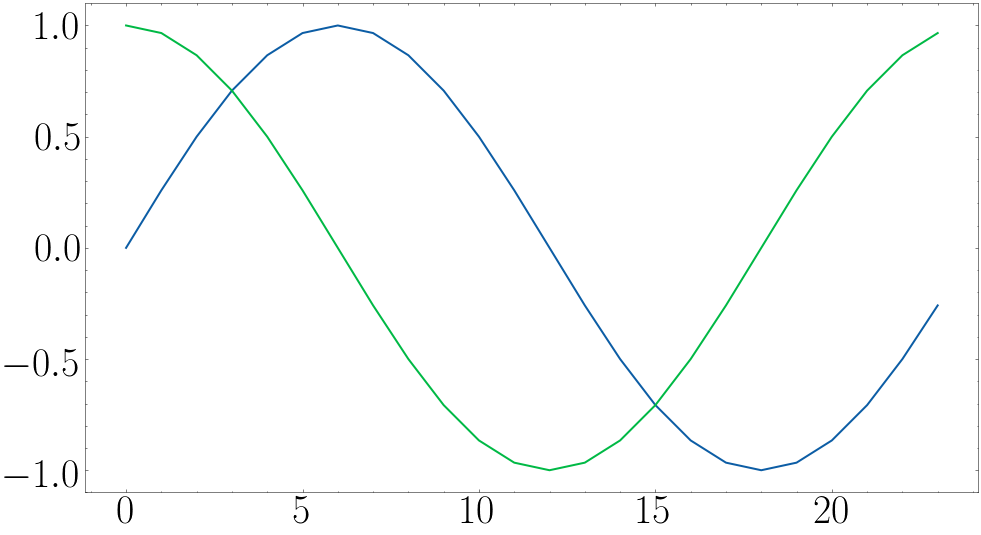
\includegraphics[width=0.4\textwidth]{images/solution/modules/hour_signal.png}\label{fig:f1}}
  \hfill
  \subfloat[Hora con valores discretos de $0$ a $23$]{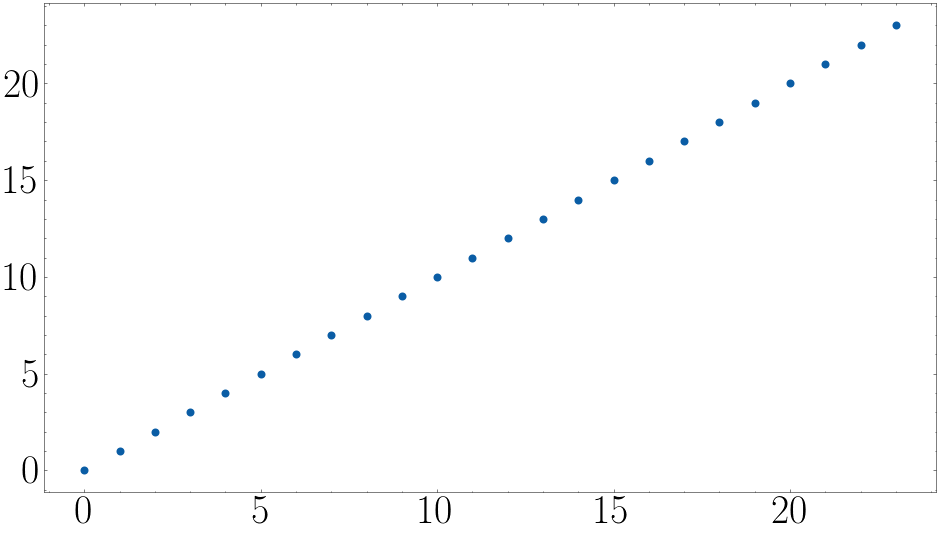
\includegraphics[width=0.4\textwidth]{images/solution/modules/hour_steps.png}\label{fig:f2}}
  \caption{Posibles formas de representar la variable \textit{hour}.}
  \label{fig:hour-stepvssignal}
\end{figure}
    
\end{enumerate}


El \small{\verb|DataFrame|} obtenido por este módulo se guarda en un fichero CSV llamado \small{\verb|intervals.csv|} que será usado por los siguientes módulos cuyo contenido tendrá una estructura similar a la que se muestra en la Tabla \ref{tab:intervals_example}.

\begin{minted}[fontsize=\footnotesize]{python}
# Save df in a CSV file
df.to_csv("path/to/intervals.csv")
\end{minted}